\documentclass[13pt,a4paper]{article}
\usepackage[utf8]{vietnam}
\usepackage{amsmath,amssymb}
\usepackage{geometry}
\geometry{top=1.5cm,bottom=1.2cm,left=1.4cm,right=1.4cm,headheight=28pt,headsep=12pt,footskip=18pt}
\usepackage{tikz}
\usepackage{xcolor}
\usepackage{graphicx}
\usepackage{fancyhdr}
\usepackage{tabularx}
\usepackage{enumitem}

\renewcommand{\baselinestretch}{1.25}
\setlength{\parskip}{2pt}
\setlength{\parindent}{0pt}

\definecolor{hfRed}{RGB}{211,47,47}
\definecolor{hfGreen}{RGB}{139,195,144}
\definecolor{myGreen}{RGB}{46,125,50}
\definecolor{myBlue}{RGB}{21,101,192}
\definecolor{mySub}{RGB}{0,105,92}

\pagestyle{fancy}
\fancyhf{}
\fancyhead[L]{\small\itshape\color{hfRed} Tài liệu lưu hành nội bộ}
\fancyhead[R]{\small\itshape\color{hfRed} Thầy \textbf{TRẦN VĂN THẠNH} - 0777.470.803}
\renewcommand{\headrulewidth}{0.8pt}
\renewcommand{\headrule}{\hbox to\headwidth{\color{hfGreen}\leaders\hrule height \headrulewidth\hfill}}

\fancyfoot[L]{\small\itshape\color{hfRed} CS1: 6/15 Nguyễn Hoàng, P. Kim Long, TP Huế \quad|\quad CS2: 24 Đặng Thái Thân, TP Huế}
\fancyfoot[R]{\small\bfseries\color{hfRed} Trang \thepage}
\renewcommand{\footrulewidth}{0.8pt}
\renewcommand{\footrule}{\hbox to\headwidth{\color{hfGreen}\leaders\hrule height \footrulewidth\hfill}}

\begin{document}

% --- TITLE BLOCK ---
\begin{tabularx}{\textwidth}{@{}l X r@{}}
\textbf{\small SỞ GIÁO DỤC VÀ ĐÀO TẠO THỪA THIÊN HUẾ} & & \textbf{\small ĐỀ CƯƠNG ÔN TẬP KIỂM TRA GIỮA KÌ I} \\
\textbf{\normalsize TRƯỜNG THCS NGUYỄN THỊ MINH KHAI} & & \textbf{\normalsize MÔN: KHOA HỌC TỰ NHIÊN 7} \\
\textit{\small (Đề cương ôn tập toàn diện)} & & \textbf{\small NĂM HỌC 2026 - 2027}
\end{tabularx}

\begin{center}
{\color{purple!80!black}\textbf{(BẢN TRÌNH CHIẾU / GIẢNG DẠY MÀN HÌNH -- CÓ CHỪA CHỖ TRỐNG)}}\par\vspace{3pt}
\textit{Họ, tên học sinh:} \dotfill \quad \textit{Lớp:} \dots\dots\dots \quad \textit{Trường:} \dotfill
\end{center}
\vspace{-4pt}
{\color{gray!50}\hrule height 0.8pt}
\vspace{8pt}

% =========================================================================
% I. KHTN (VẬT LÝ)
% =========================================================================
{\color{myGreen}\large\bfseries I. KHTN (VẬT LÝ)}

\vspace{3pt}
{\color{mySub}\textbf{A. Lý thuyết:}}

\textbf{1.} Nêu ý nghĩa của tốc độ. Tốc độ chuyển động là gì? Viết công thức tính tốc độ. Ghi chú tên và đơn vị của từng đại lượng có trong công thức.
\par\vspace{1pt}\noindent\dotfill\par\vspace{4pt}\noindent\dotfill\par\vspace{4pt}\noindent\dotfill\par\vspace{4pt}\noindent\dotfill\par\vspace{4pt}\noindent\dotfill\par\vspace{4pt}\noindent\dotfill\par\vspace{4pt}\noindent
\textbf{2.} Theo em để xác định tốc độ chuyển động người ta phải đo những đại lượng nào và dùng những dụng cụ nào để đo? Tại sao?
\par\vspace{1pt}\noindent\dotfill\par\vspace{4pt}\noindent\dotfill\par\vspace{4pt}\noindent\dotfill\par\vspace{4pt}\noindent\dotfill\par\vspace{4pt}\noindent\dotfill\par\vspace{4pt}\noindent\dotfill\par\vspace{4pt}\noindent
\textbf{3.} Nêu công dụng, cấu tạo và hoạt động của thiết bị bắn tốc độ.
\par\vspace{1pt}\noindent\dotfill\par\vspace{4pt}\noindent\dotfill\par\vspace{4pt}\noindent\dotfill\par\vspace{4pt}\noindent\dotfill\par\vspace{4pt}\noindent\dotfill\par\vspace{4pt}\noindent\dotfill\par\vspace{4pt}\noindent\dotfill\par\vspace{4pt}\noindent
\textbf{4.} Đồ thị quãng đường - thời gian cho biết gì? Đồ thị của chuyển động có tốc độ không đổi có dạng như thế nào?
\par\vspace{1pt}\noindent\dotfill\par\vspace{4pt}\noindent\dotfill\par\vspace{4pt}\noindent\dotfill\par\vspace{4pt}\noindent\dotfill\par\vspace{4pt}\noindent\dotfill\par\vspace{4pt}\noindent\dotfill\par\vspace{4pt}\noindent
\vspace{4pt}
{\color{mySub}\textbf{B. Vận dụng:}}

\textbf{1.} Một người đi bộ từ nhà ra công viên trên đoạn đường $3{,}6\text{ km}$ hết thời gian $40\text{ min}$. Tính tốc độ của người đó ra đơn vị $\text{km/h}$ và $\text{m/s}$.
\par\vspace{1pt}\noindent\dotfill\par\vspace{4pt}\noindent\dotfill\par\vspace{4pt}\noindent\dotfill\par\vspace{4pt}\noindent\dotfill\par\vspace{4pt}\noindent\dotfill\par\vspace{4pt}\noindent\dotfill\par\vspace{4pt}\noindent
\textbf{2.} Bạn Bình đi từ nhà đến trường hết $15\text{ min}$ với tốc độ $5\text{ m/s}$. Tính quãng đường từ nhà đến trường của bạn Bình ra đơn vị $\text{m}$ và $\text{km}$.
\par\vspace{1pt}\noindent\dotfill\par\vspace{4pt}\noindent\dotfill\par\vspace{4pt}\noindent\dotfill\par\vspace{4pt}\noindent\dotfill\par\vspace{4pt}\noindent\dotfill\par\vspace{4pt}\noindent\dotfill\par\vspace{4pt}\noindent
\textbf{3.} Bạn Tú đi bộ từ nhà đến thư viện lấy sách với tốc độ không đổi là $0{,}5\text{ m/s}$. Biết quãng đường từ nhà đến thư viện là $0{,}6\text{ km}$. Tính thời gian bạn Tú đi được ra đơn vị $\text{h}$ và $\text{s}$.
\par\vspace{1pt}\noindent\dotfill\par\vspace{4pt}\noindent\dotfill\par\vspace{4pt}\noindent\dotfill\par\vspace{4pt}\noindent\dotfill\par\vspace{4pt}\noindent\dotfill\par\vspace{4pt}\noindent\dotfill\par\vspace{4pt}\noindent
\textbf{4.} Một chiếc ô tô và một chiếc xe máy được phát hiện bởi thiết bị bắn tốc độ, chạy từ vạch mốc 1 và vạch mốc 2 cách nhau $5\text{ m}$, thời gian ô tô chạy giữa hai vạch mốc là $0{,}2\text{ s}$ và thời gian xe máy chạy giữa hai vạch mốc là $0{,}25\text{ s}$.
\begin{enumerate}[label=\alph*.,leftmargin=1.5cm,itemsep=1pt]
  \item Hỏi tốc độ của ô tô và của xe máy bằng bao nhiêu?
  \item Nếu tốc độ giới hạn của cung đường là $80\text{ km/h}$ thì ô tô và xe máy có vượt quá tốc độ giới hạn không? Tại sao?
\end{enumerate}
\par\vspace{1pt}\noindent\dotfill\par\vspace{4pt}\noindent\dotfill\par\vspace{4pt}\noindent\dotfill\par\vspace{4pt}\noindent\dotfill\par\vspace{4pt}\noindent\dotfill\par\vspace{4pt}\noindent\dotfill\par\vspace{4pt}\noindent\dotfill\par\vspace{4pt}\noindent\dotfill\par\vspace{4pt}\noindent
\textbf{5.} Hình dưới đây biểu diễn đồ thị quãng đường - thời gian của một vật chuyển động trong khoảng thời gian $8\text{ s}$.

\begin{center}
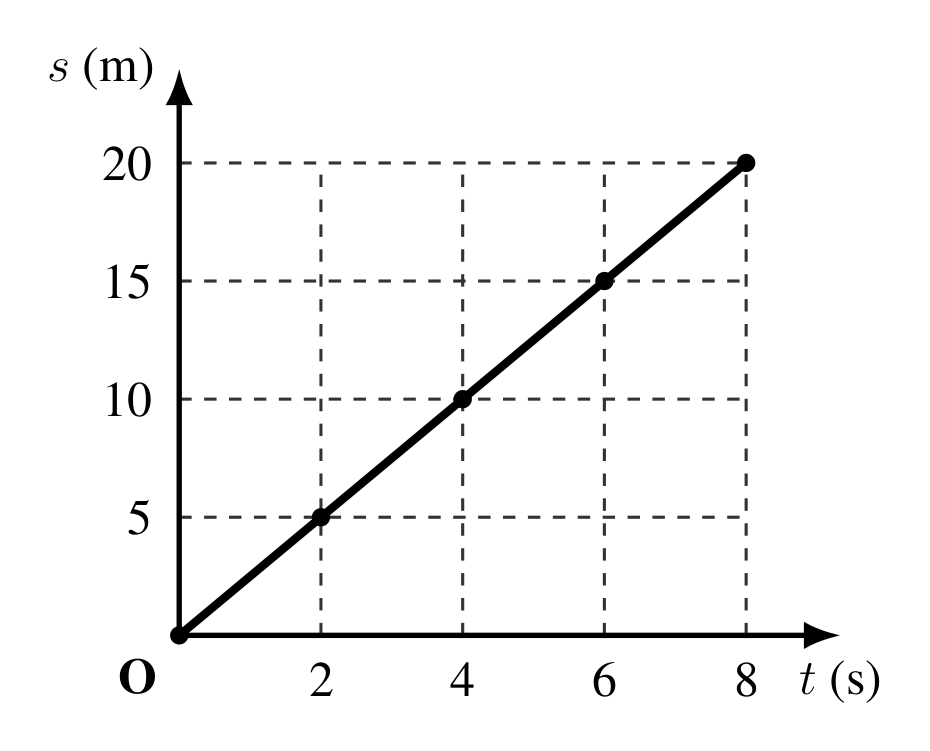
\includegraphics[width=6.5cm]{images_khtn7/do_thi_cau5.png}
\end{center}

\begin{enumerate}[label=\alph*.,leftmargin=1.5cm,itemsep=1pt]
  \item Xác định quãng đường đi được của vật sau $8\text{ s}$ kể từ lúc xuất phát.
  \item Sau bao lâu kể từ lúc xuất phát vật đi hết quãng đường $15\text{ m}$?
  \item Sau $2\text{ s}$ kể từ lúc xuất phát vật đi hết quãng đường là bao nhiêu?
  \item Từ đồ thị, hãy xác định tốc độ của vật.
\end{enumerate}
\par\vspace{1pt}\noindent\dotfill\par\vspace{4pt}\noindent\dotfill\par\vspace{4pt}\noindent\dotfill\par\vspace{4pt}\noindent\dotfill\par\vspace{4pt}\noindent\dotfill\par\vspace{4pt}\noindent\dotfill\par\vspace{4pt}\noindent\dotfill\par\vspace{4pt}\noindent
\textbf{6.} Bảng dưới đây ghi lại quãng đường đi được theo thời gian của một người đi bộ:

\begin{center}
\begin{tabular}{|l|c|c|c|c|c|c|}
\hline
\textbf{Thời gian (s)} & 0 & 10 & 20 & 30 & 40 & 50 \\ \hline
\textbf{Quãng đường (m)} & 0 & 14 & 28 & 42 & 56 & 70 \\ \hline
\end{tabular}
\end{center}

\begin{enumerate}[label=\alph*.,leftmargin=1.5cm,itemsep=1pt]
  \item Dựa vào số liệu trong bảng, hãy vẽ đồ thị quãng đường - thời gian của người đi bộ.
  \item Từ đồ thị, xác định tốc độ đi bộ của người đó.
\end{enumerate}

\begin{center}
\fbox{\parbox{0.95\textwidth}{\centering\vspace{5cm}\textit{\color{gray}[ KHUNG VẼ ĐỒ THỊ TRÊN MÀN HÌNH ]}\vspace{1cm}}}
\end{center}
\par\vspace{1pt}\noindent
\dotfill\par\vspace{4pt}\noindent\dotfill\par\vspace{4pt}\noindent\dotfill\par\vspace{4pt}\noindent\dotfill\par\vspace{4pt}\noindent
\vspace{6pt}
{\color{myGreen}\large\bfseries II. KHTN (HÓA HỌC)}

\vspace{3pt}
{\color{mySub}\textbf{A. Lý thuyết:}}

\textbf{1.} Bài 1: Phần II: Một số kĩ năng tiến trình học tập môn khoa học tự nhiên: quan sát, phân loại, liên kết, đo, dự báo.
\par\vspace{1pt}\noindent\dotfill\par\vspace{4pt}\noindent\dotfill\par\vspace{4pt}\noindent\dotfill\par\vspace{4pt}\noindent\dotfill\par\vspace{4pt}\noindent\dotfill\par\vspace{4pt}\noindent\dotfill\par\vspace{4pt}\noindent\dotfill\par\vspace{4pt}\noindent
\textbf{2.} Chương I. Nguyên tử. Sơ lược về bảng tuần hoàn các nguyên tố hóa học.
\begin{itemize}[leftmargin=*,itemsep=1pt]
  \item Trình bày được mô hình nguyên tử của Rutherford - Bohr: mô hình sắp xếp electron trong các lớp của vỏ nguyên tử, cấu tạo nguyên tử (hạt nhân và lớp vỏ nguyên tử).
  \item Nêu được khối lượng của một nguyên tử theo đơn vị quốc tế amu (đơn vị khối lượng nguyên tử), khối lượng amu các hạt proton, neutron, electron, từ đó tính khối lượng nguyên tử.
\end{itemize}
\par\vspace{1pt}\noindent\dotfill\par\vspace{4pt}\noindent\dotfill\par\vspace{4pt}\noindent\dotfill\par\vspace{4pt}\noindent\dotfill\par\vspace{4pt}\noindent\dotfill\par\vspace{4pt}\noindent\dotfill\par\vspace{4pt}\noindent\dotfill\par\vspace{4pt}\noindent\dotfill\par\vspace{4pt}\noindent
\vspace{4pt}
{\color{mySub}\textbf{B. Một số bài tập vận dụng:}}

\textbf{1.} Quan sát hình 2.1 sgk và cho biết các thành phần cấu tạo của nguyên tử.
\par\vspace{1pt}\noindent\dotfill\par\vspace{4pt}\noindent\dotfill\par\vspace{4pt}\noindent\dotfill\par\vspace{4pt}\noindent\dotfill\par\vspace{4pt}\noindent\dotfill\par\vspace{4pt}\noindent
\textbf{2.} Quan sát hình 2.2 sgk áp dụng mô hình nguyên tử của Bo, mô tả cấu tạo của nguyên tử hydrogen, và nguyên tử carbon.
\par\vspace{1pt}\noindent\dotfill\par\vspace{4pt}\noindent\dotfill\par\vspace{4pt}\noindent\dotfill\par\vspace{4pt}\noindent\dotfill\par\vspace{4pt}\noindent\dotfill\par\vspace{4pt}\noindent\dotfill\par\vspace{4pt}\noindent
\textbf{3.} Khi tìm hiểu về mô hình nguyên tử carbon theo Rutherford – Bohr, người ta xác định được hạt nhân nguyên tử chứa 6 proton, 6 neutron và vỏ nguyên tử chứa 6 electron.
\begin{enumerate}[label=\alph*.,leftmargin=1.5cm,itemsep=1pt]
  \item Ở lớp vỏ nguyên tử carbon, 6 electron được phân bố thành 2 lớp. Vẽ mô hình cấu tạo nguyên tử Carbon.
  \item Biết rằng khối lượng nguyên tử tập trung chủ yếu ở hạt nhân và coi khối lượng mỗi proton và neutron xấp xỉ 1 amu. Tính khối lượng của nguyên tử carbon bao nhiêu amu?
\end{enumerate}

\begin{center}
\fbox{\parbox{0.95\textwidth}{\centering\vspace{4.5cm}\textit{\color{gray}[ KHUNG VẼ MÔ HÌNH NGUYÊN TỬ CARBON ]}\vspace{0.8cm}}}
\end{center}
\par\vspace{1pt}\noindent
\dotfill\par\vspace{4pt}\noindent\dotfill\par\vspace{4pt}\noindent\dotfill\par\vspace{4pt}\noindent\dotfill\par\vspace{4pt}\noindent
\textbf{4.} Khi tìm hiểu cấu tạo nguyên tử nhôm (Aluminium) theo mô hình Rutherford – Bohr, học sinh xác định được trong hạt nhân nguyên tử này có 13 proton.
\begin{enumerate}[label=\alph*.,leftmargin=1.5cm,itemsep=1pt]
  \item Em hãy vẽ sơ đồ mô hình nguyên tử nhôm theo Rutherford – Bohr.
  \item Biết nhôm có khối lượng nguyên tử 27 amu, khối lượng mỗi proton và neutron xấp xỉ 1 amu. Tính số hạt neutron.
\end{enumerate}

\begin{center}
\fbox{\parbox{0.95\textwidth}{\centering\vspace{4.5cm}\textit{\color{gray}[ KHUNG VẼ MÔ HÌNH NGUYÊN TỬ NHÔM ]}\vspace{0.8cm}}}
\end{center}
\par\vspace{1pt}\noindent
\dotfill\par\vspace{4pt}\noindent\dotfill\par\vspace{4pt}\noindent\dotfill\par\vspace{4pt}\noindent\dotfill\par\vspace{4pt}\noindent
\vspace{6pt}
{\color{myGreen}\large\bfseries III. KHTN (SINH HỌC)}

\vspace{3pt}
{\color{mySub}\textbf{A. Trắc nghiệm \& Câu hỏi ôn tập trọng tâm:}}

\textbf{1.} Khái niệm, vai trò của trao đổi chất và chuyển hóa năng lượng.
\par\vspace{1pt}\noindent\dotfill\par\vspace{4pt}\noindent\dotfill\par\vspace{4pt}\noindent\dotfill\par\vspace{4pt}\noindent\dotfill\par\vspace{4pt}\noindent\dotfill\par\vspace{4pt}\noindent\dotfill\par\vspace{4pt}\noindent
\textbf{2.} Các yếu tố ảnh hưởng đến quang hợp như thế nào?
\par\vspace{1pt}\noindent\dotfill\par\vspace{4pt}\noindent\dotfill\par\vspace{4pt}\noindent\dotfill\par\vspace{4pt}\noindent\dotfill\par\vspace{4pt}\noindent\dotfill\par\vspace{4pt}\noindent\dotfill\par\vspace{4pt}\noindent
\textbf{3.} Các yếu tố ảnh hưởng đến hô hấp tế bào như thế nào?
\par\vspace{1pt}\noindent\dotfill\par\vspace{4pt}\noindent\dotfill\par\vspace{4pt}\noindent\dotfill\par\vspace{4pt}\noindent\dotfill\par\vspace{4pt}\noindent\dotfill\par\vspace{4pt}\noindent\dotfill\par\vspace{4pt}\noindent
\textbf{4.} Đặc điểm cấu tạo của lá phù hợp với chức năng quang hợp.
\par\vspace{1pt}\noindent\dotfill\par\vspace{4pt}\noindent\dotfill\par\vspace{4pt}\noindent\dotfill\par\vspace{4pt}\noindent\dotfill\par\vspace{4pt}\noindent\dotfill\par\vspace{4pt}\noindent\dotfill\par\vspace{4pt}\noindent
\textbf{5.} Khái niệm, phương trình tổng quát của quang hợp, hô hấp tế bào.
\par\vspace{1pt}\noindent\dotfill\par\vspace{4pt}\noindent\dotfill\par\vspace{4pt}\noindent\dotfill\par\vspace{4pt}\noindent\dotfill\par\vspace{4pt}\noindent\dotfill\par\vspace{4pt}\noindent\dotfill\par\vspace{4pt}\noindent
\textbf{6.} Mối quan hệ giữa tổng hợp và phân giải chất hữu cơ ở tế bào.
\par\vspace{1pt}\noindent\dotfill\par\vspace{4pt}\noindent\dotfill\par\vspace{4pt}\noindent\dotfill\par\vspace{4pt}\noindent\dotfill\par\vspace{4pt}\noindent\dotfill\par\vspace{4pt}\noindent\dotfill\par\vspace{4pt}\noindent
\textbf{7.} Ý nghĩa của việc trồng và bảo vệ cây xanh.
\par\vspace{1pt}\noindent\dotfill\par\vspace{4pt}\noindent\dotfill\par\vspace{4pt}\noindent\dotfill\par\vspace{4pt}\noindent\dotfill\par\vspace{4pt}\noindent\dotfill\par\vspace{4pt}\noindent\dotfill\par\vspace{4pt}\noindent
\vspace{4pt}
{\color{mySub}\textbf{B. Tự luận:}}

\textbf{Vận dụng hô hấp tế bào vào thực tiễn:} Giải thích vì sao rau củ quả thường được bảo quản trong ngăn mát tủ lạnh. Vì sao một số loại thực phẩm bảo quản quá lâu thì bị giảm chất lượng\dots
\par\vspace{1pt}\noindent\dotfill\par\vspace{4pt}\noindent\dotfill\par\vspace{4pt}\noindent\dotfill\par\vspace{4pt}\noindent\dotfill\par\vspace{4pt}\noindent\dotfill\par\vspace{4pt}\noindent\dotfill\par\vspace{4pt}\noindent\dotfill\par\vspace{4pt}\noindent\dotfill\par\vspace{4pt}\noindent\dotfill\par\vspace{4pt}\noindent\dotfill\par\vspace{4pt}\noindent
\end{document}
